\begin{figure}[htbp]
\centering
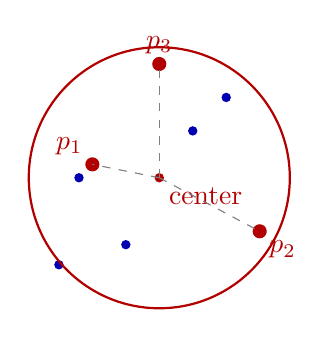
\begin{tikzpicture}[scale=0.85]
  \foreach \x/\y in {1/2, 2/3.5, 3.5/1, 0.5/0.5, 3/3, 1.5/0.8, 2.5/2.5, 0.8/1.8} {
    \fill[blue!70!black] (\x,\y) circle (2pt);
  }
  \fill[red!70!black] (1,2) circle (3pt) node[above left] {$p_1$};
  \fill[red!70!black] (3.5,1) circle (3pt) node[below right] {$p_2$};
  \fill[red!70!black] (2,3.5) circle (3pt) node[above] {$p_3$};
  \draw[thick,red!70!black] (2,1.8) circle (1.95);
  \fill[red!70!black] (2,1.8) circle (2pt) node[below right] {center};
  \draw[gray,dashed] (2,1.8)--(1,2);
  \draw[gray,dashed] (2,1.8)--(3.5,1);
  \draw[gray,dashed] (2,1.8)--(2,3.5);
\end{tikzpicture}
\caption{Welzl's algorithm: the smallest enclosing circle is defined by at most 3 support points (red).}
\label{fig:welzl}
\end{figure}
